% id: 1124
% book: RPM 공통수학2 · 10 무리함수
% section: 시험에 꼭 나오는 문제
% figure: crop:fig-1124.png
% answer: ①
% answer_source: 답지
% variant_level: 0 (원본 전사)
% 이 파일은 build.mjs 가 items.json 에서 만든다. 고칠 때는 items.json 을 고친다.
\hspace*{2mm}\begin{minipage}[t]{\dimexpr\linewidth-2mm\relax}\vspace{0pt}\smash{\raisebox{1.5mm}{\dmkichul{RPM 공통수학2 1124번 · 164쪽}}}
\noindent\begin{minipage}[t]{0.58\linewidth}\vspace{0pt}\raggedright 함수 $y=\dfrac{a}{x+b}+c$의 그래프가 오른쪽 그림과 같을 때, 다음 중 함수 $y=\sqrt{ax+b}+c$의 그래프가 지나는 사분면만을 모두 고른 것은? \cond{$a$, $b$, $c$는 상수이다.}\end{minipage}\hfill\begin{minipage}[t]{0.4\linewidth}\vspace{0pt}\centering 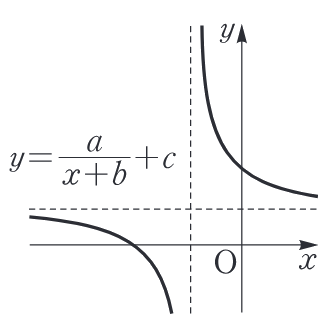
\includegraphics[width=78.3pt]{figures/fig-1124.png}\end{minipage}\par
\begin{choicesii}{제$1$, $2$사분면}{제$3$, $4$사분면}{제$1$, $2$, $3$사분면}{제$1$, $2$, $4$사분면}{제$1$, $3$, $4$사분면}\end{choicesii}\end{minipage}
